\chapter{Przygotowany system sterowania ruchem}
System, przygotowany do badania algorytmu sterowania, składa się z trzech podstawowych komponentów:
\begin{description}
	\item[symulator] --
		symuluje ruch drogowy, udostępnia dane z czujników i przyjmuje ustawienia sygnalizatorów.
		Jest on również źródłem czasu co pozwala na synchronizację działania całego systemu. Opisany w rozdziale \ref{chap:symulacja}.
	\item[kontroler] --
		osobny dla każdego obszaru, otrzymuje dane z symulatora i wyznacza sterowania sygnalizatorów.
		Może komunikować się z innymi kontrolerami w celu wymiany danych o sąsiednich obszarach. Więcej w sekcji \ref{chap:kontroler}.
	\item[serwer] --
		zapewnia abstrakcję komunikacji. Pozwala na wymiane wiadomości w postaci zdarzeń.
		Działanie komunikacji w systemie opisane jest w sekcji \ref{chap:komunikacja}.
\end{description}

\section{Technologia}
System został przygotowany przy użyciu języka C++ w standardzie C++03 z wykorzystaniem biblioteki Boost 1.55.0 \cite{boost}. Do komunikacji sieciowej wykorzystano bibliotekę Google Protocol Buffer \cite{protobuf}. Przygotowane testy jednostkowe wykorzystują bibliotekę Google Test \cite{gtest}.

Obszar symulowany wczytywany jest z plików XML z opisem w postaci grafowej. Pliki z opisem zawierają również obliczone czasy międzyzielone pomiędzy kolizyjnymi strumieniami ruchu.

\section{Kontroler}
\label{chap:kontroler}
Kontroler został przygotowany do działania z różnymi, prostymi w modyfikacji, algorytmami sterowania. Zmiana wybranego algorytmu spośród zaimplementowanych odbywa się poprzez edycję pliku konfiguracyjnego. Dla celu badań przygotowany został, poza opisanym algorytmem, algorytm sterowania przy użyciu stałoczasowego, wczytywanego z pliku, programu sygnalizacji.

\section{Komunikacja}
\label{chap:komunikacja}
Symulowany system sterowania ruchem wykorzystuje komunikację sieciową do połączenia komponentów. W założeniu wdrożony system wykorzystywałby czujniki i kontrolery komunikujące się przy użyciu sieci ethernet. Przygotowany, symulowany, system wykorzystuje do komunikacji centralny serwer odpowiedzialny za wymianę zdarzeń pomiędzy komponentami przy użyciu dyspozytora zdarzeń. Komunikacja sieciowa odbywa się przy użyciu biblioteki protobuf \cite{protobuf} w celu serializacji i deserializacji wiadomości.

\chapter{Symulator ruchu drogowego}
\label{chap:symulacja}
\section{Obszar badania algorytmu}
Dla celów badania algorytmu przygotowany został opis obszaru okolic placu Grunwaldzkiego we Wrocławiu, przedstawionego na rysunku \ref{fig:mapa_czysta}.

\begin{figure}[h]
    \centering
    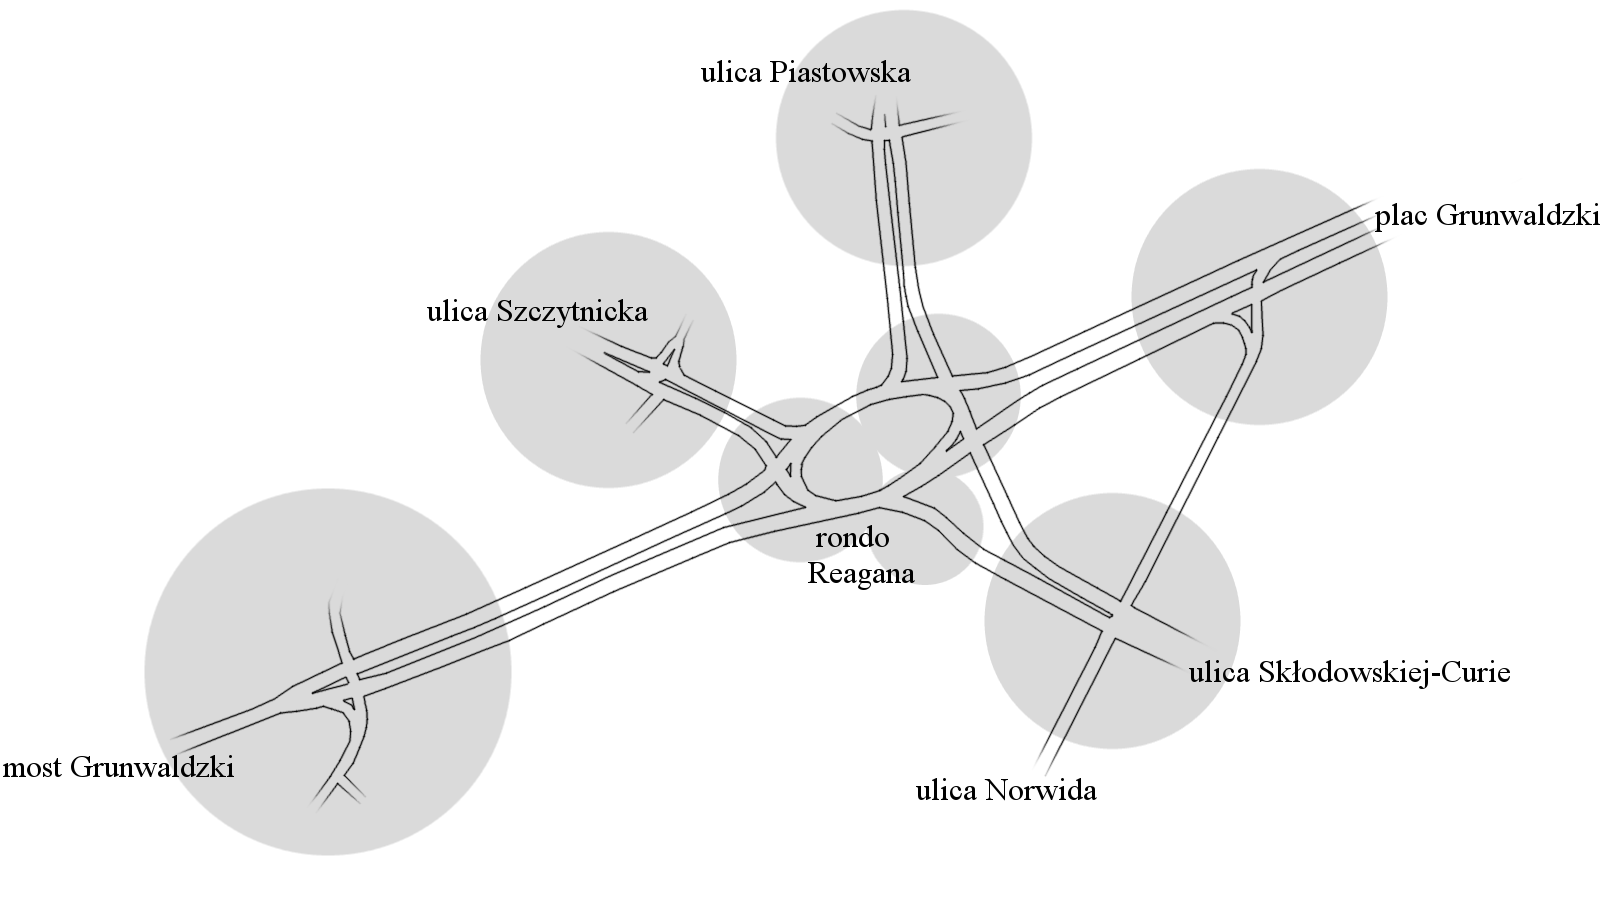
\includegraphics[width=1.0\textwidth]{images/mapa_czysta.png}
    \caption{Mapa obszaru badania algorytmu przedstawiająca okolice placu Grunwaldzkiego we Wrocławiu, przygotowana na podstawie Google Maps \cite{google_maps}}
    \label{fig:mapa_czysta}
\end{figure}

Przygotowany obszar został oparty o rzeczywisty układ drogowy, jednakże został on uproszczony. Uwzględnia on jedynie ruch samochodowy, nie uwzględnia natomiast komunikacji miejskiej czy ruchu pieszego. Takie też zastosowanie ma opracowywany algorytm sterowania.

Sterowany obszar podzielony został na osiem autonomicznych obszarów oznaczonych na rysunku \ref{fig:mapa_czysta}. Każdy z tych obszarów jest sterowany przez osobny kontroler.

Model sterowanego obszaru generowany jest w postaci komórkowej, wymaganej przez symulator, na podstawie przygotowanego opisu obszaru w postaci grafowej.

\section{Symulator}
Dla celów wykonania badań przygotowany został symulator oparty o model Nagela - Schreckenberga, powszechnie znany jako model NaSch, opisany w pracy z 1992 roku \cite{nasch}. Model ten działa w oparciu o automat komórkowy i cztery proste fazy ruchu.

Automat komórkowy stworzony przez Nagela i Schreckenberga wykorzystuje jednowymiarową tablicę komórek, gdzie każda z nich może pomieścić jeden pojazd. Wszystkie pojazdy poruszają się w tym samym kierunku z maksymalną prędkością 5 komórek na sekundę. W każdym kroku symulacji, na wszystkich pojazdach, wykonywane są 4 fazy ruchu:

\begin{itemize}
	\item przyspieszenie
	\item spowolnienie
	\item losowość
	\item ruch
\end{itemize}

Pierwsza faza, faza przyspieszenia, oznacza zwiększenie prędkości każdego pojazdu, ale nie przekraczając maksymalnej dozwolonej prędkości.
Prędkość pojazdu wyrażana jest w liczbie komórek na sekundę.
\begin {equation}
	v_{faza_1} = min (v(n) + 1, v_{max})
\end {equation}

W drugiej fazie ruchu wykonywane jest spowolnienie spowodowane innymi pojazdami. Jeśli pojazd widzi inny pojazd, przed nim, w odległości mniejszej niż jego prędkość, redukuje on swoją prędkość do wielkości odstępu.
\begin {equation}
	v_{faza_2} = max (v_{faza_1}, odstep)
\end{equation}

W kolejnej fazie, z pewnym ustalonym prawdopodobieństwem, generowane jest spowolnienie poruszających się pojazdów.
\begin {equation}
	\begin{array} {c}
		v(n+1) = v_{faza_2} - 1\\
		\textrm{lub}\\
		v(n+1) = v_{faza_2}
	\end{array}
\end{equation}

Ostatnią fazą jest faza ruchu. Każdy z pojazdów jest przesuwany o, ustaloną w poprzednich fazach, liczbę komórek.

Podstawową zaletą tak zdefiniowanego modelu jest prostota jego implementacji i dokładność wystarczająca do badania zachowanie ruchu drogowego w różnych sytuacjach, co opisuje w swojej pracy Maciej Bartodziej \cite{bartodziej}. W swoich badaniach prezentuje on również możliwości prostych modyfikacji modelu, co jest istotne w przypadku przygotowywanego symulatora.

Model NaSch prezentuje również pewne ograniczenia. Przede wszystkim jest on modelem dyskretnym, upływ czasu odzwierciedlany jest w postaci stanów dyskretnych. Jednocześnie pozycja pojazdów jest ograniczona do pojedynczych komórek. Ze względu na domyślną wielkość komórki o wartości 7,5 metra, prędkość pojazdów może przyjąć jedną z kilku wartości: 0, 7,5, 15 i 22,5 metra na sekundę, czyli odpowiednio 0, 27, 54 i 81 kilometrów na godzinę. Dla celów pracy magisterskiej przyjęta została maksymalna prędkość trzech komórek na sekundę -- 81 kilometrów na godzinę.

\begin{figure}[h]
    \centering
    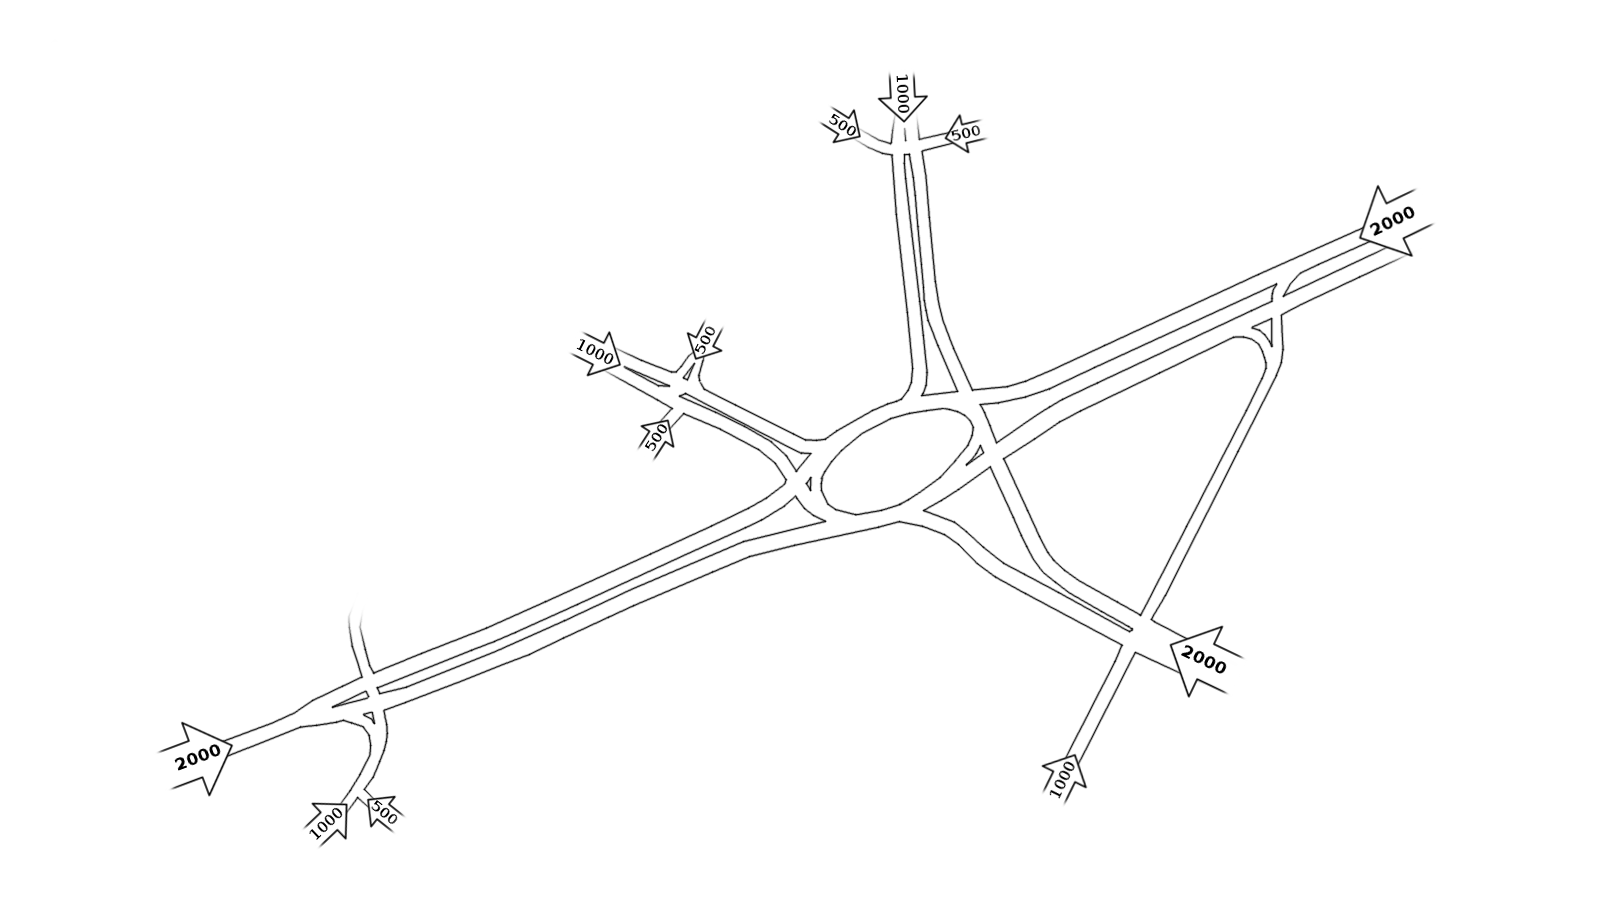
\includegraphics[width=1.0\textwidth]{images/mapa_ruch.png}
    \caption{Mapa przepływu pojazdów (w pojazdach na godzinę) w punktach wejściowych do sterowanego obszaru, przygotowana na podstawie Google Maps \cite{google_maps}}
    \label{fig:mapa_ruch}
\end{figure}

Na potrzeby symulacji ruchu na przedstawionym obszarze model NaSch został zmodyfikowany w celu przystosowania go do działania z przecinającym się ruchem na skrzyżowaniach i obsługę sterowania ruchem. Model został zmodyfikowany poprzez:
\begin{itemize}
	\item usunięcie fazy losowości ze względu na chęć badania reakcji ruchu na zmiany w sterowaniu nie losową charakterystykę ruchu,
	\item wprowadzenie elementów tworzących pojazdy zgodnie z przyjętym przepływem na punktach wejściowych do sterowanego obszaru,
	\item dodanie możliwości sterowania sygnałem zezwalającym na opuszczenie komórki i reakcja pojazdów na nadawane synały,
	\item modyfikacja fazy spowolnienia dla uwzględnienia konieczności zatrzymania się przed przecinającym strumieniem ruchu, w celu eliminacji blokowania innych pojazdów,
\end{itemize}

Ze względu na przedstawione ogranicznia symulatora, przyjęte zostały orientancyjne wartości przepływów pojazdów w punktach wejściowych, przedstawione na rysunku \ref{fig:mapa_ruch}.

Symulatowane są również czujniki ruchu. Czujnik przepływu pojazdów oblicza aktualny przepływ pojazdów na podstawie liczby pojazdów które przecięły określoną komórkę w ciągu ostatnich 10 sekund (jest to parametr konfiguracyjny symulatora). Czujnik kolejki określa wielkość kolejki na wyznaczonym odcinku, przez zliczenie liczby pojazdów znajdujących się w komórkach danego odcinka. Symulowane czujniki odzwierciedlają kamery z oprogramowaniem pozwalającym na wykrywanie pojazdów i pętle indukcyjne montowane w jezdni.

Symulator jest głównym źródłem czasu dla pozostałych komponentów systemu. Udostępnia on sygnał zegarowy o okresie jednej sekundy co wyzwala wyznaczenie nowego stanu sygnalizatorów przez kontrolery. Sygnał zegarowy jest odpowiednikiem sygnału 1PPS\footnote{one pulse per second (jeden impuls na sekundę) - elektroniczny sygnał synchronizacyjny, udostępniany między innymi przez satelity GPS} stosowanego powszechnie do synchronizacji działania układów elektronicznych.
